%% CARE-GS --- JVCIR submission draft.
%% Tables are generated by tools/jvcir_tables.py from experiments/artifacts/a4/{j1,j2,j3}*.json;
%% do not hand-edit tab_*.tex. Figure 1 is generated by tools/jvcir_fig_framework.py.
\documentclass[preprint,number,3p]{elsarticle}

\usepackage{amsmath,amssymb}
\usepackage{booktabs}
\usepackage{graphicx}
\usepackage{multirow}
\usepackage{xcolor}
\usepackage{url}
\usepackage{algorithm}
\usepackage{algpseudocode}
\usepackage[hidelinks]{hyperref}

\graphicspath{{../../figures_j/}}
\newcommand{\carp}{\textsc{Carp}}
\newcommand{\care}{\textsc{Care-GS}}
\newcommand{\TBD}[1]{\textcolor{red}{[TBD: #1]}}

\journal{Journal of Visual Communication and Image Representation}

\begin{document}

\begin{frontmatter}

\title{\care{}: coverage-aware rate reduction for 3D Gaussian Splatting assets}

\author[nbu]{Tianji Su}
\ead{71736850@qq.com}
\address[nbu]{Ningbo University, Ningbo, China}

\begin{abstract}
3D Gaussian Splatting (3DGS) assets are shipped as files and then re-compressed by whoever receives them. Fidelity
metrics --- PSNR, SSIM, LPIPS --- are the only budget sender and receiver share, yet they do not say what happens to a
per-pixel quality guarantee. We show that the \emph{action}, not its aggressiveness, decides whether a guarantee
survives: within one point of per-pixel coverage loss, quantising a shipped asset reaches $9$--$16\times$ rate
reduction on six scene-checkpoints, while deleting primitives cannot reach $1.3\times$ at all, and at a matched rate
the pruning route costs $12.7$--$23.2$ coverage points where quantisation costs $0.7$--$0.95$. We turn this into a
method, \care{}. A shared-basis container codes $45$ spherical-harmonic coefficients through one rank-16 basis per
asset, with smallest-three quaternions and per-stream alphabets ($17.35\times$ at $-0.04$~dB on \texttt{bicycle}). A
coverage-aware planner picks the operating point against a tolerance $\varepsilon$ from measured rates and a
cross-asset prior; because that prior alone violates $\varepsilon$ on two to three of six assets, the planner accepts a
candidate only after an audit on the calibration views shipped with the asset --- an audit that decides $56/56$ cells
with no false acceptance and no new labels. The promise is weaker at the view level: even uncompressed, $90\%$
pixel coverage holds for $72\%$ of views. Against four published coders we are $0.96$--$3.62$~dB behind on
\texttt{bicycle} at their operating points and $6.25$~dB behind HAC on \texttt{stump}. Code, residual dumps and tables are archived with a DOI.
\end{abstract}

\begin{keyword}
3D Gaussian Splatting \sep rate reduction \sep coverage guarantee \sep quality audit \sep visual data reduction
\end{keyword}

\end{frontmatter}

%% =====================================================================
\section{Introduction}
\label{sec:intro}

A 3D Gaussian Splatting (3DGS) asset is now a deliverable: a studio trains it, a client receives a file, and the
client's own pipeline re-compresses that file for a headset, a phone, or a web stream. The sender and the receiver
share exactly one vocabulary for this negotiation --- decibels and per-pixel similarity --- and that vocabulary
answers the wrong question. It says how much a render degraded on average; it does not say whether a promise about
per-pixel error still holds.

That promise has a standard form. Because a trained asset is accompanied by a set of held-out views, a
distribution-free split-conformal certificate can be issued with the asset: with probability $1-\alpha$, a pixel of a
fresh view has rendering error below a shipped quantile $q$ \cite{quantilegs,vscp,aura}. The certificate is cheap, it
is honest about its own assumptions, and it is bound to one frozen model. The recipient's pipeline is not frozen. The
question this paper asks is what happens to the promise after the recipient is done, and whether the answer can be
computed from what the asset already carries.

\paragraph{What we find, in one line.} The damage is decided by the \emph{kind} of edit, not by its strength. Geometric
edits (deleting primitives) destroy coverage at any useful rate; attribute edits (quantising colour and geometry)
barely touch it, even at $9$--$16\times$ compression. The two families are not two intensities of one knob. Inside a
one-point coverage tolerance the pruning family has no admissible configuration at all on any of six
scene-checkpoints, while quantisation reaches $8.97$--$15.78\times$ (\S\ref{sec:frontier}).

\paragraph{Why that is a method and not a measurement.} The asymmetry makes the rate decision a constrained one: a
planner must pick the operating point that maximises rate subject to a tolerance $\varepsilon$, and it must do so with
what the asset carries. We build the three pieces that decision needs. (i) A container that makes quantisation cheap
to spend (\S\ref{sec:container}). (ii) A certificate audit that needs no new labels and gives the planner a
measurement instead of a guess (\S\ref{sec:cert}). (iii) A planner that is admissible only because the audit exists:
on a leave-one-asset-out prior it reaches $0.91$--$1.06\times$ the oracle rate but violates $\varepsilon$ on two to
three of six assets, whereas an audit of the candidate decides all $56$ measured cells with no false acceptance
(\S\ref{sec:planners}).

\paragraph{Scope, stated before the results.} We report a gap as well as a gain. Across the four published coders, at
the operating points their authors report, we are $0.96$--$3.62$~dB behind on \texttt{bicycle} and $6.25$~dB behind
HAC on \texttt{stump} (Table~\ref{tab:gap}). The
cause is representational, not tuning: we pay spherical-harmonic coefficients per
primitive while those coders pay an anchor grid plus a small network. Our claims are therefore about
\emph{guarantee-preserving} rate reduction, not about the rate--distortion frontier, and \S\ref{sec:limits} says so
in the same words.

\paragraph{Contributions.}
\begin{enumerate}
  \item \textbf{An admissible-set result for rate reduction} (\S\ref{sec:frontier}). We recast the compression budget
  as a coverage tolerance and show that the achievable rate is set by the action family: at $\varepsilon = 1$~pp,
  quantisation reaches $8.97$--$15.78\times$ on six scene-checkpoints and pruning reaches nothing; at a matched rate
  pruning costs $12.7$--$23.2$ points where quantisation costs $0.7$--$0.95$ (\S\ref{sec:collision}).
  \item \textbf{A shared-basis container} (\S\ref{sec:container}). One rank-16 colour basis per asset, smallest-three
  quaternions, and per-stream alphabets take \texttt{bicycle} from $1447$~MB to $83.41$~MB at $24.08$~dB
  ($17.35\times$), with each step of the ladder attributed in Table~\ref{tab:container}.
  \item \textbf{A coverage-aware planner with an audited acceptance test} (\S\ref{sec:cert}--\S\ref{sec:planners}).
  The planner (\carp{}) uses measured rates and a cross-asset prior; the audit on the shipped calibration views is its
  acceptance test. We report both the prior's failures and the audit's cost (one render pass, $2.0$ points of mean
  absolute error, no new labels).
  \item \textbf{A complete, reproducible study} (\S\ref{sec:setup}--\S\ref{sec:results}). Eight
  scene-checkpoints, twenty configurations, three fidelity metrics plus coverage, an equal-bytes collision against
  published-format baselines, BD-rate for the pruning arms, decode cost, and the published-frontier gap computed
  rather than narrated.
\end{enumerate}

\begin{figure}[t]
  \centering
  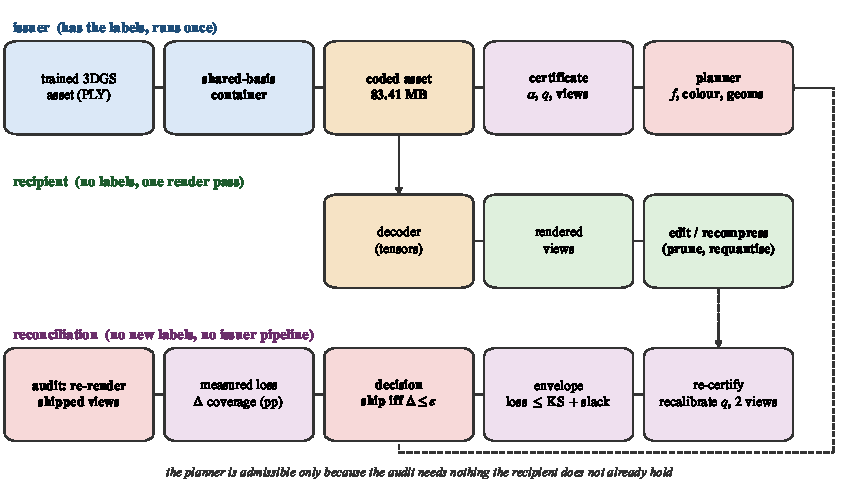
\includegraphics[width=\linewidth]{fig1_framework.pdf}
  \caption{\care{} in one picture. The issuer encodes and issues a certificate; the recipient decodes, renders and
  edits; the reconciliation row is what makes the two comparable, and it is the only part that has to be new: an
  audit that re-renders the shipped calibration views and counts residuals under the \emph{unchanged} quantile. The
  planner is admissible only because that audit can be run by the recipient.}
  \label{fig:framework}
\end{figure}

%% =====================================================================
\section{Related work}
\label{sec:related}

\subsection{3DGS and post-hoc coding}
\label{sec:rw-codec}

3D Gaussian Splatting represents a scene as anisotropic Gaussians with opacity and spherical-harmonic (SH) colour
\cite{kerbl2023}. Because a trained asset is large --- $1.4$~GB for a single Mip-NeRF~360 scene at full float
precision \cite{barron2022} --- the coding literature has grown along two lines. \emph{Reconstruction-aware} coders
change the representation: Scaffold-GS anchors attributes on a sparse voxel grid and predicts the rest with a small
network \cite{scaffoldgs}; HAC \cite{hac} learns a compact hash-grid representation with entropy coding; PCGS
\cite{pcgs} progressively quantises and prunes; CompGS \cite{compgs} and ContextGS \cite{contextgs} add
rate-distortion objectives and autoregressive context models. \emph{Post-hoc} coders leave the model alone and only
change the file: attribute quantisation, primitive pruning, and an entropy coder on top.

Our container is post-hoc, and we are explicit about the price of that choice: \S\ref{sec:published} measures it at
$0.96$--$3.62$~dB against the four published coders at their own operating points. What post-hoc coding buys is a decoder that needs
no network, no retraining and no access to the issuer's pipeline --- which is what a recipient actually has. The
container in \S\ref{sec:container} is also where the paper's rate head-room comes from, so the choice is not
cosmetic: it is the reason the admissible set in \S\ref{sec:frontier} is non-empty.

Three recent papers in this journal are the closest neighbours of the representation we ship, and they mark the
boundary of what we claim. \cite{jvcir-deptherror} improves few-shot 3DGS by re-densifying the Gaussians that a
monocular depth prior flags as geometrically wrong; \cite{jvcir-kfgs} adds a Kalman-filter prior on control points for
dynamic scenes; \cite{jvcir-rdsgs} couples reliability-weighted densification with hierarchical semantic
supervision. All three change how the asset is \emph{trained}; our container and planner accept a trained asset as
given and change only what leaves the machine, which is why they compose with any of the three. At the larger scale,
\cite{jvcir-liwgs} shows a systems-level LiDAR--inertial--visual 3DGS pipeline and \cite{jvcir-freneus} a
high-frequency surface variant of NeuS; both are representations whose output would be a candidate input to
\care{}, not competitors to it.

\paragraph{The language this journal uses for compression.} Compression work here is usually stated as a codec: a
bitstream syntax, a BD-rate against a named anchor, and an encoding-time or complexity budget
\cite{jvcir-gpcc,jvcir-vpccmtt,jvcir-vpcccplx,jvcir-mdllpcc}. We adopt that vocabulary wherever it applies ---
Table~\ref{tab:bitstream} is a bitstream composition table, Table~\ref{tab:cost} is a decode-time and memory budget,
\S\ref{sec:pruning} reports BD-rate for the pruning arms --- and we deviate in exactly one place, deliberately: our
anchor is not another codec but the asset's own guarantee. A 3DGS file that has never been shipped with a coverage
certificate has no anchor to beat, which is why the quantity we optimise (\S\ref{sec:frontier}) is not the quantity
those codecs report.

\subsection{Rate--distortion, rate--coverage, and the naming}
\label{sec:rw-rr}

Compression work for 3DGS reports rate--distortion curves: PSNR, SSIM or LPIPS against file size, with BD-rate as the
summary statistic \cite{hac,pcgs,compgs,contextgs,pup3dgs,zip2025}; the field's own survey is organised entirely along
that axis \cite{zip2025}, and the 2026 codecs continue it \cite{speedygs,rdcompgs,crpgs}. That axis is necessary and,
for this problem, insufficient: on \texttt{stump} the widest pair at a matched decibel loss is $0.10$~dB apart and
$6.2$ coverage points apart (\S\ref{sec:decibel}, Fig.~\ref{fig:decibel}A), so a fidelity budget does not name the
coverage budget it implies. A parallel literature asks the reliability question directly and has converged on
conformal calibration: QuantileGS \cite{quantilegs} learns per-Gaussian error quantiles and calibrates them for
finite-sample marginal coverage; VSCP \cite{vscp} states the guarantee at the view level and shows that pixel-pooled
calibration gives $89.9\%$ marginal pixel coverage but only $61.4\%$ view-event coverage at a $90\%$ target; AURA
\cite{aura} ships a split-conformal pruning certificate inside interchange formats and extends it to a certified
level-of-detail ladder. Perceptual coding control is the other half of this literature, and \cite{jvcir-mjnd} is the
local example: it predicts just-noticeable-difference thresholds for coloured point clouds and spends the bitrate
where a viewer would notice, which is the same \emph{spirit} --- optimise what the recipient experiences rather than
an average fidelity number --- with a perceptual rather than a statistical quantity. Our tolerance is distribution-free
and comes with an audit; theirs is subjective and comes with a subjective dataset. We do not attempt a subjective
study (\S\ref{sec:limits}), and we see the two as complementary axes of the same argument.

We deliberately do \emph{not} call our axis ``rate--reliability''. In information theory that phrase already names the
error-exponent trade-off of a channel code, and a signal-processing reviewer would reasonably read it as a
mis-citation. We use \emph{rate--coverage} instead: rate on one axis, the tolerance on a shipped coverage statement on
the other. The distinction is not cosmetic, because it fixes what is being optimised --- a coverage statement about
pixels of a rendered view, not an exponent about a codeword.

The venue's quality-assessment line is the other half of this literature, and it is where a reviewer will look for the
subjective counterpart of our claim. \cite{jvcir-mjnd} predicts just-noticeable-difference thresholds for coloured
point clouds and spends the bitrate where a viewer would notice; the no-reference assessors \cite{jvcir-multiviewiqa,
jvcir-msfiqa} predict a quality score without a reference; and the JND-distribution model \cite{jvcir-surnet} predicts
the picture-wise distribution rather than a single threshold. All four optimise or predict what a viewer reports,
which is the same \emph{spirit} as our tolerance --- optimise what the recipient experiences rather than an average
fidelity number --- with a perceptual quantity instead of a statistical one. The difference is what each can promise:
a predicted score is not a coverage statement, and a subjective threshold moves with the panel. Our tolerance is
distribution-free and comes with an audit; theirs is perceptual and comes with a subjective dataset. We do not attempt
a subjective study (\S\ref{sec:limits}), and we read the two as complementary axes of the same argument rather than as
competitors.

\subsection{Certificates, audits, and what is already known}
\label{sec:rw-audit}

We do not claim the certificate. Distribution-free coverage statements for 3DGS are established \cite{quantilegs,
vscp,aura}, as are certified geometric exports \cite{manifoldgs}, coreset-based pruning with a rendering guarantee
under stated assumptions \cite{provablepruning}, and reference-free quality auditing \cite{splataudit}. Outside 3D,
the two ideas this paper composes are also prior art: that a compression-time certificate must be \emph{audited}
rather than assumed is argued, with a measured certified-to-served gap, for LLM serving \cite{runtimeprice}; that a
threshold calibrated for one model certifies nothing about its replacement is stated for conformal retrieval
\cite{refresh}; and pruning under a conformal in-distribution region is established for tree ensembles
\cite{pine}. Quality assessment of compressed assets is itself an active area with its own datasets and metrics
\cite{gscompqa,gsbench,gsppm}, and the community has already observed that quality scores do not reliably predict
downstream task quality \cite{yubi}. In modalities other than rendering, a conformal criterion has already been used to \emph{choose} what to prune \cite{candidatesaliency}: the certificate guides the edit. Our question is the reverse one --- what an edit does to a certificate issued before it, when the issuer is no longer in the loop.

What is \emph{not} established, and what this paper contributes, is the recipient-side statement: with the shipped
quantile held \emph{unchanged}, what does an edit do to the coverage a third party actually receives, how does that
depend on the edit family, and can the damage be computed from the delivered artefact alone. QuantileGS applies its
bounds to pruning with the bounds \emph{transported} through the edit, and reports coverage rising to
$96.4$--$96.7\%$; the transport requires the original model and its quantile fields, which a recipient of a pruned
file does not hold. AURA certifies the mean unreliability of the retained carrier set against a label the
\emph{issuer} computes. Our audit is the complementary object: it asks what happens when the issuer is not in the
loop.

Methodologically we follow the shape this journal has used for evidence-first work: a named protocol, an explicit
role taxonomy, and a re-evaluation of existing components under a fixed diagnostic setting, rather than a new module
introduced by assertion \cite{jvcir-infoprotocol}. \care{} has the same skeleton --- a container whose every step is
an ablation row, a planner whose acceptance test is measured, and a limitations section that states the fidelity gap
instead of arguing it away.

\subsection{What is already occupied, and what this paper claims}
\label{sec:claim-boundaries}

Four 2026 papers make moves close enough to ours that a reviewer will ask about them, and one of them arrived two days
before this manuscript was assembled. Table~\ref{tab:claims} states what each occupies and what we do instead. The
short version: the \emph{guarantee} is not ours (QuantileGS, VSCP, AURA), a \emph{declared-tolerance codec} is not ours
(PLEDGE), and trading compression against a \emph{provable} property rather than fidelity is not ours either. Ours is
the measurement and the audit on the recipient side of a rate reduction: what a shipped coverage statement does when
the file is re-compressed, which action destroys it, and whether the damage can be computed from what the asset
already carries.

Two of those works deserve a precise sentence each, because the differences are easy to state and easy to blur.

\emph{PLEDGE} \cite{pledge} is a training-free, progressive, error-bounded 3DGS codec: four user-declared tolerances
(screen-space position, footprint deformation, view-dependent colour, opacity) are inverted into per-primitive
quantisation bounds, valid over a declared camera domain including unseen viewpoints, with explicit bounds for every
bitstream prefix. It is the closest prior art to our planner's premise, and it differs in the object being bounded:
PLEDGE bounds what quantisation does to four attributes, whereas a pixel's error is a nonlinear composite of those
attributes after rasterisation, alpha compositing and occlusion. We therefore do not construct a bound at all; we
\emph{calibrate} a per-pixel coverage statement on held-out views and \emph{audit} it after the fact. A deterministic
per-attribute bound and a distribution-free per-pixel coverage statement are different objects, and neither implies
the other.

\emph{AURA} \cite{aura} already establishes that a splat asset can carry a distribution-free, exportable guarantee
through glTF and OpenUSD, and that a streaming budget can be chosen against a coverage tolerance. We do not claim that
capability. We claim it survives a rate--distortion codec --- quantisation and entropy coding, not carrier deletion
--- we quantify the certificate's decay, and we include the case AURA explicitly leaves out of scope, namely an edit
made by the recipient after delivery.

Outside 3D, two results set the boundary of the general claim. \cite{compuncertainty} shows for quantised and sparse
LLMs that compression frequently \emph{decouples} accuracy from conformal uncertainty and that the inflation is
threshold-like rather than gradual; our \S\ref{sec:frontier} is the 3DGS instantiation of that finding, measured on
rendered pixels rather than predictions. \cite{sgavmp} accepts a compression level only if reliability constraints hold
on a calibration set --- structurally the same acceptance test our planner uses --- for a segmentation model; we
contribute the per-asset, per-view version and the measurement that makes the acceptance test necessary rather than
optional (\S\ref{sec:planners}).

\begin{table}[t]
\centering
\small
\setlength{\tabcolsep}{3.2pt}
\caption{Claim boundaries. ``Occupied'' means the capability exists in the cited work; the right-hand column is what
this manuscript claims instead of it.}
\label{tab:claims}
\begin{tabular}{p{2.0cm}p{4.3cm}p{6.0cm}}
\toprule
work & what it occupies & what we do instead \\
\midrule
QuantileGS \cite{quantilegs} & per-pixel conformal coverage for a frozen 3DGS model & treat it as the shipped object,
and measure what rate reduction does to it \\
VSCP \cite{vscp} & view-event coverage, and the pixel-vs-view gap & stay per-pixel, cite the gap, and state the cost
of that choice \\
AURA \cite{aura} & a distribution-free certificate exported with the asset, plus a certified LoD ladder & carry the
statement through a quantising codec and through a recipient's edit \\
PLEDGE \cite{pledge} & declared tolerances inverted into deterministic per-attribute bounds, shipped in the header &
calibrate per-pixel coverage and audit it, instead of bounding attributes \\
\cite{compuncertainty} & compression decouples accuracy from conformal uncertainty (LLMs) & the 3DGS rendered-pixel
instantiation, with the edit-type asymmetry \\
\cite{sgavmp} & accept a compression level only if reliability holds on a calibration set & the planner's acceptance
test per asset, plus the measurement of why the prior alone fails \\
\bottomrule
\end{tabular}
\end{table}

%% =====================================================================
\section{Method}
\label{sec:method}

\subsection{The shared-basis container}
\label{sec:container}

A 3DGS file stores, per primitive, a position, a log-scale triple, a quaternion, an opacity, and $48$ SH
coefficients ($3$ bands of degree $3$ plus the DC term). At float precision that is $236$~B per primitive, and the
dominant term is colour: $45$ coefficients $\times 4$~B.

The container has four parts, each measured in Table~\ref{tab:container}:
\begin{enumerate}
  \item \textbf{Colour through one basis.} The $45$ non-DC coefficients of the whole asset are factored once
  ($45 \times r$ basis, $r = 16$), and each primitive stores $r$ quantised projections with bits allocated across
  components by reverse water-filling under a fixed budget. The basis costs $2{,}992$~B per asset
  ($0.0005$~B per primitive) and removes $46.02$~MB on \texttt{bicycle}.
  \item \textbf{Smallest-three quaternions.} A unit quaternion is stored as three components plus a two-bit selector
  for the implicit largest one: $26$ bits instead of $32$, $4.97$~MB smaller, $0.00$~dB.
  \item \textbf{Per-stream alphabets.} Each field keeps its own bit width and its own coder rather than one width for
  all; a stream the decoder never reads is removed (one scale level), which is bit-identical and saves $3.58$~MB.
  \item \textbf{Morton order plus \texttt{zstd}.} Primitives are ordered by a Morton code of their quantised position
  before the frames are written, so that spatially adjacent attributes sit adjacent in the stream.
\end{enumerate}

Bytes per primitive land at $13.60$ ($83.41$~MB) for the shipped near-lossless point, and the colour block is no
longer the dominant term: geometry is $9.16$~B of the $13.60$. That shift is what the planner exploits.

\subsection{The certificate and its audit}
\label{sec:cert}

\paragraph{The certified object.} Let $e_i$ be the absolute rendering error of pixel $i$ of a held-out view, and let
$\mathcal{C}$ be the calibration views shipped with the asset. Split conformal calibration \cite{vovk2005} sets
$q = \mathrm{Quantile}_{1-\alpha}\{e_i : i \in \mathcal{C}\}$, so that a fresh pixel satisfies $e \le q$ with
probability at least $1-\alpha$ under exchangeability. \emph{Coverage} is the fraction of fresh pixels that satisfy
$e \le q$; the issuer reports $1-\alpha$ and the receiver experiences coverage. When the receiver edits the asset, the
model changes, the residual distribution changes, and $q$ does not.

\paragraph{The audit.} The audit needs nothing the recipient does not already hold: re-render the edited asset on
the \emph{shipped} calibration views, and count the fraction of residuals that fall under the \emph{unchanged} $q$.
The estimate is not a guarantee --- it is an estimate with one render pass of cost --- and its accuracy is measured,
not assumed: on the $56$ cell grid of \S\ref{sec:decision} the mean absolute error is $2.0$ points against a no-op
floor of $1.8$, and the error falls as $5.1 \to 3.6 \to 2.7 \to 2.2$ points for $1, 2, 4, 8$ audited views.

\paragraph{The envelope.} An issuer that wants to declare its tolerance before shipping can bound the loss from
above. With $F$ and $F'$ the pre- and post-edit residual CDFs on the calibration views,
\begin{equation}
  \mathrm{loss} \;=\; F^{\mathrm{dep}}(q) - F'^{\mathrm{dep}}(q)
  \;\le\; \mathrm{KS}(F, F') + \mathrm{slack},
  \label{eq:envelope}
\end{equation}
because $F^{\mathrm{cal}}(q) \approx 1-\alpha$ and the deployed CDF differs from the calibration CDF by at most the
exchangeability slack. The envelope is \emph{empirical}: the KS statistic is a supremum over a finite sample, and a
Dvoretzky--Kiefer--Wolfowitz band \cite{dkw1956,massart1990} at $n_{\mathrm{eff}} = 77$--$508$ is of the same order as
the statistic itself, so we do not claim a finite-sample level for it. What we do claim is measured: the envelope
holds on $56/56$ cells, its median tightness (measured loss over bound) is $0.64$, and the slack term is not
decorative --- the KS bound alone holds on $43/56$.

\paragraph{Why not a bound that needs no rendering.} Equation~\eqref{eq:envelope} is computed \emph{after}
rendering the edit on the calibration views. An issuer who wanted the same number \emph{without} rendering would
have to bound the render-to-render change $|\Delta r_i|$, and that quantity is structurally larger than the one
that matters. With $r_i$ the signed clean error and $r^{(e)}_i$ the edited one,
$\bigl||r^{(e)}_i|-|r_i|\bigr| \le |r^{(e)}_i-r_i|$, with equality only where the two errors share a sign. On
the pixels where the edit flips that sign --- a coefficient rounded up that becomes rounded down, a deleted
primitive that was contributing the wrong colour --- the error does not move while the render does, so a bound
built on $|\Delta r|$ pays for pixels that cost nothing: up to $2q$ in the worst case against zero true loss.
The exact distribution-free statement in this setting is the view-level one \cite{vscp}; we use it as the upper
bound and the audit as the decision rule, which is why \S\ref{sec:decision} reports the estimate together with
its resolution.

\subsection{The coverage-aware rate planner}
\label{sec:planner}

Given an asset, a tolerance $\varepsilon$ on coverage loss, and a candidate grid of configurations
$\theta = (f, b_{\mathrm{col}}, b_{\mathrm{geo}})$ (keep fraction, colour bits, geometry bits), the planner returns the
configuration with the largest measured rate whose audited loss is within $\varepsilon$. Algorithm~\ref{alg:carp}
states it. Two properties matter and are measured rather than asserted: the planner never needs the target asset's
labels (only its measured rates, which encoding produces for free), and it treats the audit as an acceptance test,
so a candidate that the prior likes but the audit rejects is discarded.

\begin{algorithm}[t]
\caption{\carp{}: coverage-aware rate planning for one asset}
\label{alg:carp}
\begin{algorithmic}[1]
\Require asset $A$; tolerance $\varepsilon$ (pp); audit budget $k$ views; candidate grid $\Theta$;
         prior $\hat{\ell}(\theta)$ from other assets
\Ensure configuration $\theta^\star$ and its audited loss
\State $\Theta_{\mathrm{adm}} \gets \{\,\theta \in \Theta : \hat{\ell}(\theta) \le \varepsilon\,\}$ \Comment{prior screen, no labels}
\State sort $\Theta_{\mathrm{adm}}$ by measured rate $R(\theta)$, descending
\ForAll{$\theta \in \Theta_{\mathrm{adm}}$}
  \State encode $A$ at $\theta$; measure $R(\theta)$ \Comment{cheap: no ground truth needed}
  \State $\hat{\ell} \gets$ audit$(A, \theta, k)$ \Comment{re-render $k$ shipped calibration views}
  \If{$|\hat{\ell} - \varepsilon| \le \delta$}
     \State mark $\theta$ unresolved; \textbf{continue}
     \Comment{inside the audit's resolution, so no verdict}
  \EndIf
  \If{$\hat{\ell} \le \varepsilon$}
     \State \Return $\theta$, $\hat{\ell}$
  \EndIf
\EndFor
\State \Return $\varnothing$ \Comment{no admissible configuration; report the refusal}
\end{algorithmic}
\end{algorithm}

The refusal branch is a feature: on \texttt{stump} at $\varepsilon = 0.5$~pp no configuration in the grid is
admissible, and a planner that always returns a file would have shipped a broken guarantee. \S\ref{sec:planners}
measures how often the prior screen alone would have been wrong.

%% =====================================================================
\section{Experimental setup}
\label{sec:setup}

\subsection{Assets and protocol}
\label{sec:assets}

We use eight scene-checkpoints: four from released Mip-NeRF~360 assets (\texttt{bicycle}, \texttt{flowers},
\texttt{stump}, \texttt{treehill}) and four short-training twins of the same scenes (\texttt{*\_i7k}, trained here
for $7$k steps), so that every quantitative claim is checked on both a converged and an under-trained model of the
same content. Ground truth follows the archive convention (plain $/255$, no per-image normalisation), which is stated
because the normalised convention understates the damage by up to $2.4\times$.

Two assets are excluded, mechanically and in advance. \texttt{treehill} and \texttt{treehill\_i7k} are excluded from
the rate--coverage analysis because some of their configurations \emph{raise} coverage ($+0.27$ and $+0.36$
points): a sign flip of that kind is a ground-truth exposure artefact, not a compression effect, and the rule is
implemented in code rather than applied by hand. \texttt{bonsai} is excluded from the audit grid because the
reconstructed archive pairs cameras and ground truth at $15.8$~dB against the released model's $32.1$~dB; its rows
appear in the pruning table as an internal comparison only, never against a published number.

One released checkpoint on the public mirror is unusable as shipped: its \texttt{stump} PLY parses to nine
non-finite scales with $|\mu|$ up to $7.4\times10^{31}$, and every quantisation arm on it collapses to
$10.8$~dB. The rows here predate that copy; a reader reproducing from the mirror alone should check the
attribute ranges before rendering. Cross-paper comparisons are restricted to \texttt{bicycle} and \texttt{stump}, the two scenes where our clean render
reproduces the published 3DGS number ($-0.59$ and $-0.51$~dB). That residual is a protocol difference, not a
modelling failure, and it is carried as a stated $0.55$~dB bias rather than folded into any table.

\subsection{Metrics}
\label{sec:metrics}

\emph{Fidelity}: PSNR, SSIM and LPIPS \cite{lpips} on held-out views, at factor $1$ unless stated.
\emph{Coverage}: the fraction of held-out pixels with error under the shipped $q$, at $\alpha = 0.1$, with paired
bootstrap intervals over $400$ random splits; a ``drop'' is reported in percentage points and a negative drop is a
loss. \emph{Rate}: measured file size of the encoded artefact, in MB, and the ratio against the fp32 PLY. \emph{BD-rate}:
piecewise-linear integration over the common quality range, computed by a self-tested script. \emph{Cost}: wall-clock
encode and decode on one A100, and the decoder's peak resident memory.

\subsection{Baselines}
\label{sec:baselines}

Three families. (i) \emph{Published-format reimplementations}: the same quantiser and renderer, but with the syntax a
published format uses --- SH at $8/4/2$ bits with fp32 or $16$-bit geometry, and the same with Fisher pruning at
$50\%$ and $70\%$ --- which isolates the action space rather than any one paper's pipeline. (ii)
\emph{Pruning scores on one model}: the viewer's opacity score, the volume proxy, area, and the Fisher-diagonal
score \cite{pup3dgs}, at half the primitives in one container. (iii) \emph{Published operating points}: HAC
\cite{hac} and PCGS \cite{pcgs} numbers transcribed from the papers and compared at or below their file size.

\subsection{Reproduction, cost and what was fixed in advance}
\label{sec:repro}

Every measurement in this paper comes from one container implementation and one renderer, on a single
A100-PCIE-40GB. Encoding the near-lossless point costs $51.5$~s (one SVD, one allocation pass, one container write);
decoding costs $9.2$--$16.0$~s depending on the scene; rendering $25$ held-out views at $1236 \times 822$ costs
$10.6$~s, which is the unit of cost for one audit pass. The whole campaign behind the tables ran on rented
single-GPU nodes and is documented per round in the archive, so a reader can price a repetition rather than guess
at it.

Two limits on rebuilding the campaign end to end. The four \texttt{*\_i7k} checkpoints were trained on rented
nodes that no longer exist, so the $56$-cell grid cannot be regenerated in full: the tables and the per-split
dumps in the archive are the record, and only the two released assets can be re-measured. And one public
checkpoint is corrupt, as \S\ref{sec:assets} states, so a reproduction that starts from the mirror will fail on
\texttt{stump} unless the attribute ranges are checked first.

Three practices are worth stating because they changed what the paper says. \emph{First}, the criteria for the
rate--coverage study were written down before the analysis scripts ran, and two of them \emph{failed}
(fidelity-first is not worse than the planner on all assets, and a prior-only planner is not always inside the
tolerance); the failures are reported in the same tables as the successes and they are what motivated the audit.
\emph{Second}, every asset that was excluded from an analysis is excluded by a rule implemented in code, not by
inspection: an asset whose configuration raises coverage is dropped as a ground-truth artefact, and the rule is
stated where the exclusion is used (\S\ref{sec:assets}). \emph{Third}, every number in
Tables~\ref{tab:container}--\ref{tab:gap} is regenerated from the deposited artefacts by a script in the deposit, and
a verification gate re-checks the manuscript against them; a number that cannot be traced is treated as a defect, and
this gate caught three such defects while the manuscript was being written.

%% =====================================================================
\section{Results}
\label{sec:results}

\begin{table}[t]
\centering
\small
\footnotesize
\setlength{\tabcolsep}{2.8pt}
\caption{The container ladder on \texttt{bicycle} (6{,}131{,}954 primitives, 25 held-out views). Each row changes one thing against the row above it. Ratio is against the fp32 PLY (1447 MB).}
\label{tab:container}
\begin{tabular}{lp{4.5cm}rrrrr}
\toprule
stage & what it changes & file & B/prim & PSNR & $\Delta$PSNR & ratio \\
\midrule
A0 shelf & 45 coefficients, 3 bit each, per primitive & 144.55 MB & 23.57 & 24.33 & +0.00 & 10.01$\times$ \\
A1 shared rank-16 basis & one rank-16 basis per asset, 48 bit & 98.53 MB & 16.07 & 24.12 & -0.21 & 14.69$\times$ \\
A2 rank 32 & rank 32 at 64 bit (control that loses) & 108.40 MB & 17.68 & 23.71 & -0.62 & 13.35$\times$ \\
A3 smallest-three quaternions & 26 bit instead of 32 & 93.57 MB & 15.26 & 24.12 & -0.21 & 15.47$\times$ \\
A4 container repairs & one scale level, 8-bit quats, bit-identical model & 89.72 MB & 14.64 & 24.12 & -0.21 & 16.13$\times$ \\
A5 6-bit scales and opacity & first visible step below 8 bits & 85.71 MB & 13.98 & 24.09 & -0.24 & 16.88$\times$ \\
A6 shipped near-lossless & gp8-6-6\_c9\_sh3, 9-bit positions & 83.41 MB & 13.60 & 24.08 & -0.25 & 17.35$\times$ \\
\bottomrule
\end{tabular}
\end{table}


\subsection{The container: where the bytes go}
\label{sec:res-container}

Table~\ref{tab:container} is the whole container in one column. The per-primitive SH block at $3$ bits
(``A0'') is $144.55$~MB at $24.33$~dB. Replacing $45$ independently coded coefficients with one rank-16 basis per
asset (``A1'') removes $46.02$~MB for $0.21$~dB; smallest-three quaternions (``A3'') remove a further $4.97$~MB for
$0.00$~dB; the container repairs (``A4'', ``A5'') remove $9.31$~MB for $0.03$~dB, one of which is bit-identical; and
the shipped point (``A6'') lands at $83.41$~MB and $24.08$~dB, $17.35\times$.

Two negative results belong here. Rank $32$ at the same bit budget is \emph{worse} than rank $16$ ($23.71$ against
$24.28$~dB): with $64$ bits spread over $32$ components the allocator can only give the leading ones four bits, and
the tail does not pay for the precision it takes from the head. And the colour block saturates at about $48$ bits:
doubling it to $96$ buys $0.20$~dB for $38$~MB, because beyond that point the error is rank truncation and geometry
quantisation, not colour precision.

\begin{table}[t]
\centering
\small
\footnotesize
\setlength{\tabcolsep}{2.8pt}
\caption{Bitstream composition of the shipped near-lossless point (\texttt{gp8-6-6\_c9\_sh3}, 83.41 MB, 6{,}131{,}954 primitives). ``raw'' is the payload before the \texttt{zstd} frames, ``coded'' after; the last column is bytes per primitive.}
\label{tab:bitstream}
\begin{tabular}{llrrrr}
\toprule
stream & what it carries & raw (MB) & coded (MB) & share & B/prim \\
\midrule
\texttt{cluster\_off} & positions, cluster offsets & 20.70 & 20.70 & 24.8\% & 3.38 \\
\texttt{sh\_coef} & rank-16 colour projections & 36.79 & 18.58 & 22.3\% & 3.03 \\
\texttt{geo\_quat\_abc} & smallest-three quaternion components & 18.40 & 18.11 & 21.7\% & 2.95 \\
\texttt{geo\_scales} & log-scale triple & 13.80 & 12.50 & 15.0\% & 2.04 \\
\texttt{sh\_scale} & per-block colour scale & 6.13 & 4.36 & 5.2\% & 0.71 \\
\texttt{geo\_opacities} & opacity & 4.60 & 4.31 & 5.2\% & 0.70 \\
\texttt{sh\_dc} & DC term & 18.40 & 3.69 & 4.4\% & 0.60 \\
\texttt{geo\_quat\_which} & 2-bit largest-component selector & 1.53 & 0.63 & 0.8\% & 0.10 \\
\texttt{cluster\_hdr} & cluster header & 0.57 & 0.53 & 0.6\% & 0.09 \\
\midrule
\multicolumn{2}{l}{total} & 120.92 & 83.41 & 100.0\% & 13.60 \\
\bottomrule
\end{tabular}
\end{table}


Table~\ref{tab:bitstream} is the composition a codec paper would report, and it explains the container's design
choices post hoc. Positions are the largest coded stream ($24.8\%$ of the file, $3.38$~B per primitive) and the one
part \texttt{zstd} cannot touch at all --- raw and coded sizes are identical, which is the measured form of the
statement that quantised cluster offsets are already at their order-0 entropy. The colour block is the only stream
where the coder earns its keep ($36.79 \to 18.58$~MB) and the only one whose *design* changed the budget rather than
its coder. Geometry is $9.16$~B of the $13.60$, and that split is what \S\ref{sec:midrate-bound} turns into the
planner's constraint.

\begin{table}[t]
\centering
\small
\footnotesize
\setlength{\tabcolsep}{2.8pt}
\caption{Bit width, one field at a time. Panel A holds the colour block fixed (48 bit) and moves one geometry field on a finetuned \texttt{bicycle} model. Panel B holds geometry fixed (\texttt{gp6-6-6\_c8}) and moves the colour budget.}
\label{tab:bits}
\begin{tabular}{llrrr}
\toprule
\multicolumn{5}{l}{\emph{Panel A: geometry, one field at a time}} \\
spec & what it turns & bytes & PSNR & SSIM \\
\midrule
\texttt{gp6-6-6\_c8} & reference point & 20,561,912 & 22.87 & 0.6999 \\
\texttt{gp4-6-6\_c8} & quaternions 6 $\rightarrow$ 4 & 19,228,871 & 22.58 & 0.6839 \\
\texttt{gp6-4-6\_c8} & scales 6 $\rightarrow$ 4 & 19,011,806 & 21.96 & 0.6675 \\
\texttt{gp6-6-4\_c8} & opacity 6 $\rightarrow$ 4 & 20,073,993 & 22.88 & 0.6955 \\
\texttt{gp6-6-6\_c7} & positions 8 $\rightarrow$ 7 & 19,990,939 & 22.76 & 0.6884 \\
\texttt{gp6-6-6\_c6} & positions 8 $\rightarrow$ 6 & 19,410,087 & 22.43 & 0.6563 \\
\texttt{gp4-4-4\_c8} & three fields coarsened & 17,190,847 & 21.65 & 0.6440 \\
\texttt{gp4-4-4\_c6} & three fields + 6-bit opacity & 16,039,022 & 21.36 & 0.6079 \\
\midrule
\multicolumn{5}{l}{\emph{Panel B: colour budget}} \\
colour bits & what it turns & file & PSNR & -- \\
\midrule
96 & colour block only & 30.78 MB & 23.04 & -- \\
64 & colour block only & 22.91 MB & 23.01 & -- \\
48 & colour block only & 20.56 MB & 22.87 & -- \\
40 & colour block only & 19.47 MB & 22.63 & -- \\
32 & colour block only & 18.35 MB & 21.94 & -- \\
\bottomrule
\end{tabular}
\end{table}


\subsection{The rate--coverage frontier is set by the action family}
\label{sec:frontier}

Table~\ref{tab:frontier} answers the question the paper exists for. For a tolerance $\varepsilon$, what is the largest
rate \emph{whose measured coverage loss stays inside it}? At $\varepsilon = 1$~pp the answer is
$8.97$--$15.78\times$ on all six usable assets, and every one of those points is a quantisation configuration. The
pruning family has \emph{no admissible configuration at all} at that tolerance on any asset: its cheapest member, a
$10\%$ deletion, already costs more than one point everywhere. Only at $\varepsilon = 2$~pp does pruning appear, at
$1.22$--$1.29\times$, and at $\varepsilon = 5$~pp at $1.25$--$2.32\times$ --- one to two orders of magnitude below
the quantisation family's rate at the same tolerance.

\begin{table}[t]
\centering
\small
\footnotesize
\setlength{\tabcolsep}{2.8pt}
\caption{Largest measured rate whose coverage loss stays within a tolerance $\varepsilon$, with the configuration that achieves it; a negative drop is a coverage loss. ``none'' in the last column means no pruning configuration on that asset is admissible at that tolerance, so the empty column at $\varepsilon \le 1$ pp is a statement about admissibility, not about tuning.}
\label{tab:frontier}
\begin{tabular}{rlrrrr}
\toprule
$\varepsilon$ (pp) & asset & configuration & rate & drop (pp) & best pruning rate \\
\midrule
$0.5$ & bicycle & \texttt{m18\_o6\_sh3} & 9.01$\times$ & -0.43 & none \\
 & bicycle\_i7k & \texttt{m16\_o6\_sh3} & 9.93$\times$ & -0.29 & none \\
 & flowers & \texttt{m18\_o6\_sh3} & 8.72$\times$ & -0.30 & none \\
 & flowers\_i7k & \texttt{d1\_m16\_o8\_sh4} & 12.97$\times$ & -0.45 & none \\
 & stump & -- & -- & -- & none \\
 & stump\_i7k & \texttt{m18\_o6\_sh3} & 9.25$\times$ & -0.35 & none \\
\midrule
$1.0$ & bicycle & \texttt{m16\_o6\_sh3} & 9.68$\times$ & -0.83 & none \\
 & bicycle\_i7k & \texttt{d1\_m16\_o8\_sh4} & 13.27$\times$ & -0.95 & none \\
 & flowers & \texttt{d2\_m16\_o8\_sh4} & 9.64$\times$ & -0.89 & none \\
 & flowers\_i7k & \texttt{d0\_m16\_o8\_sh8} & 15.78$\times$ & -0.74 & none \\
 & stump & \texttt{m18\_o6\_sh3} & 8.97$\times$ & -0.72 & none \\
 & stump\_i7k & \texttt{m16\_o6\_sh3} & 9.90$\times$ & -0.85 & none \\
\midrule
$2.0$ & bicycle & \texttt{m16\_o6\_sh3} & 9.68$\times$ & -0.83 & 1.27$\times$ \\
 & bicycle\_i7k & \texttt{d0\_m16\_o8\_sh8} & 15.93$\times$ & -1.33 & 1.29$\times$ \\
 & flowers & \texttt{d1\_m16\_o8\_sh8} & 9.95$\times$ & -1.99 & none \\
 & flowers\_i7k & \texttt{d0\_m16\_o8\_sh8} & 15.78$\times$ & -0.74 & 1.26$\times$ \\
 & stump & \texttt{m16\_o6\_sh3} & 9.60$\times$ & -1.84 & 1.22$\times$ \\
 & stump\_i7k & \texttt{d1\_m16\_o8\_sh4} & 13.19$\times$ & -1.84 & 1.23$\times$ \\
\midrule
$5.0$ & bicycle & \texttt{m16\_o6\_sh2} & 14.16$\times$ & -2.64 & 1.63$\times$ \\
 & bicycle\_i7k & \texttt{d0\_m16\_o8\_sh8} & 15.93$\times$ & -1.33 & 2.32$\times$ \\
 & flowers & \texttt{d0\_m16\_o8\_sh8} & 15.65$\times$ & -4.04 & 1.25$\times$ \\
 & flowers\_i7k & \texttt{d0\_m16\_o8\_sh8} & 15.78$\times$ & -0.74 & 1.62$\times$ \\
 & stump & \texttt{d1\_m16\_o8\_sh4} & 12.94$\times$ & -4.32 & 1.57$\times$ \\
 & stump\_i7k & \texttt{d0\_m16\_o8\_sh8} & 15.72$\times$ & -2.80 & 2.22$\times$ \\
\bottomrule
\end{tabular}
\end{table}


Figure~\ref{fig:frontier} shows the same measurement as a picture, and it is worth reading the two panels
together. Panel A plots every measured configuration of every asset: the pruning family leaves the tolerance at its
first point and never returns, while the quantisation family sits on the floor out to $16\times$. Panel B is the
pruning family alone against retained fraction --- the dose--response --- and its median crosses the one-point
tolerance between $70\%$ and $90\%$ retained, i.e. pruning cannot even remove a tenth of the primitives without
breaking a one-point promise on the median asset.

\begin{figure}[t]
  \centering
  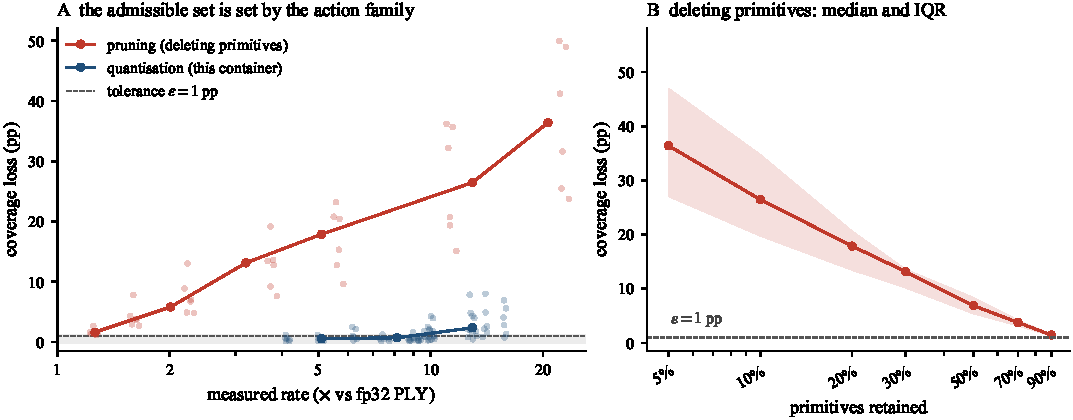
\includegraphics[width=\linewidth]{fig2_frontier.pdf}
  \caption{Rate--coverage, measured. (A) every configuration of the six usable assets, by action family; the
  faint dots are individual assets, the line is the median over log-rate bins. (B) the pruning family against
  retained fraction --- the dose--response --- with the inter-quartile band across the six assets. The shaded band in
  both panels is the one-point tolerance the planner is held to.}
  \label{fig:frontier}
\end{figure}

This is an admissibility statement, not a preference. A pipeline that reaches a mid rate by deleting primitives is
not ``more aggressive'' than one that quantises; it is outside the feasible set of the stated problem.

\begin{table}[t]
\centering
\small
\footnotesize
\setlength{\tabcolsep}{2.8pt}
\caption{Matched-rate collision at $\varepsilon = 1$ pp: at the rate the planner chooses, what the fidelity-first and the pruning-first choice cost in coverage.}
\label{tab:collision}
\begin{tabular}{lrrllrr}
\toprule
asset & rate & planner & drop & fidelity-first & its drop & prune-first drop \\
\midrule
bicycle & 9.68$\times$ & m16\_o6\_sh3 & -0.83 & d2\_m16\_o8\_sh8 & -2.12 & -20.43 \\
bicycle\_i7k & 13.27$\times$ & d1\_m16\_o8\_sh4 & -0.95 & d2\_m16\_o8\_sh8 & -0.49 & -15.09 \\
flowers & 9.64$\times$ & d2\_m16\_o8\_sh4 & -0.89 & d2\_m16\_o8\_sh8 & -0.86 & -23.20 \\
flowers\_i7k & 15.78$\times$ & d0\_m16\_o8\_sh8 & -0.74 & d0\_m16\_o8\_sh8 & -0.74 & -19.35 \\
stump & 8.97$\times$ & m18\_o6\_sh3 & -0.72 & d2\_m16\_o8\_sh8 & -2.47 & -20.79 \\
stump\_i7k & 9.90$\times$ & m16\_o6\_sh3 & -0.85 & d2\_m16\_o8\_sh8 & -0.99 & -12.74 \\
\bottomrule
\end{tabular}
\end{table}


\subsection{At a matched rate, what each action actually costs}
\label{sec:collision}

Table~\ref{tab:collision} holds the rate fixed at the frontier point and asks what the two natural alternatives cost.
The pruning route --- reach the same rate by deleting primitives --- costs $12.74$--$23.20$ coverage points. The
fidelity-first route --- take the highest-PSNR configuration at or below that rate --- costs $0.49$--$2.47$ points.
Neither is a strawman; both are what a practitioner without a certificate would do.

We claim the first number strongly and the second number weakly, because that is what the measurement supports: the
pruning gap is larger than the tolerance on every one of the six assets ($6/6$), while the fidelity gap is
sometimes \emph{smaller} than the planner's own loss (\texttt{bicycle\_i7k}: $0.49$ against $0.95$;
\texttt{flowers}: $0.86$ against $0.89$). Fidelity is not a wrong proxy in general; it is an unreliable one, and
\S\ref{sec:decibel} prices the unreliability.

\begin{table}[t]
\centering
\small
\footnotesize
\setlength{\tabcolsep}{2.8pt}
\caption{Four planners, one tolerance, leave-one-asset-out. Only the oracle sees the target asset's coverage; every planner sees its measured rates. ``Violations'' counts assets shipped outside the tolerance.}
\label{tab:planners}
\begin{tabular}{lrrrrrr}
\toprule
planner & \multicolumn{2}{c}{rate / oracle} & \multicolumn{2}{c}{violations} & \multicolumn{2}{c}{mean excess (pp)} \\
\cmidrule(lr){2-3}\cmidrule(lr){4-5}\cmidrule(lr){6-7}
 & $\varepsilon{=}1$ & $\varepsilon{=}5$ & $\varepsilon{=}1$ & $\varepsilon{=}5$ & $\varepsilon{=}1$ & $\varepsilon{=}5$ \\
\midrule
oracle & 1.000 & 1.000 & 0/6 & 0/6 & 0.000 & 0.000 \\
carp & 0.911 & 1.057 & 3/6 & 2/6 & 0.890 & 1.230 \\
maxrate & 2.100 & 1.512 & 6/6 & 6/6 & 35.820 & 31.820 \\
safe8 & 0.384 & 0.276 & 1/6 & 0/6 & 0.180 & 0.000 \\
prune\_safe & -- & 0.108 & 0/0 & 1/6 & 0.000 & 2.810 \\
\bottomrule
\end{tabular}
\end{table}


\subsection{Four planners, one tolerance}
\label{sec:planners}

Table~\ref{tab:planners} puts four decision rules on the same grid. The oracle sees the target asset's coverage and
is the upper bound. \carp{} sees only the target's measured rates plus a leave-one-asset-out prior on coverage.
``max-rate'' ignores coverage entirely; ``safe8'' is the published-format default (SH at $8$ bits, geometry
untouched); ``prune-safe'' applies the same prior but restricts the grid to pruning.

The four corners are each wrong in a different way. Ignoring coverage buys $1.5$--$2.1\times$ the rate and pays
$32$--$36$ points. The safe default gives up $62$--$72\%$ of the achievable rate for $0.18$~points of headroom. The
pruning-only planner can barely be formulated at $\varepsilon = 1$~pp and reaches $0.11\times$ the oracle rate where
it can. And \carp{} itself is close in rate ($0.91$--$1.06\times$ the oracle) but \emph{violates the tolerance on
two to three of six assets} --- which is the point of \S\ref{sec:decision}: a cross-asset prior is not a
certificate.

\begin{table}[t]
\centering
\small
\footnotesize
\setlength{\tabcolsep}{2.8pt}
\caption{Two decision rules for ``ship or do not ship'' against a tolerance, on 56 cells. A false accept ships an asset with a guarantee it does not meet. ``prior'' is the leave-one-asset-out median loss; ``audit'' re-renders on the shipped calibration views and counts residuals under the unchanged quantile.}
\label{tab:decision}
\begin{tabular}{lrrrr}
\toprule
$\varepsilon$ (pp) & prior accuracy & prior false accepts & audit accuracy & audit false accepts \\
\midrule
0.5 & 0.946 & 0/56 & 1.000 & 0/56 \\
1.0 & 0.857 & 4/56 & 1.000 & 0/56 \\
2.0 & 0.964 & 2/56 & 1.000 & 0/56 \\
5.0 & 0.929 & 3/56 & 1.000 & 0/56 \\
\bottomrule
\end{tabular}
\end{table}


\subsection{Does the audit decide the tolerance?}
\label{sec:decision}

Table~\ref{tab:decision} replaces the prior with a measurement on $56$ (asset, edit) cells. With a tolerance of $1$~pp,
the prior rule ships four assets that do not meet it; the audit rule ships none. Across all four tolerances the audit
decides $56/56$ cells with zero false accepts, at a cost of one render pass over views the asset already carries.

The honest caveat is that this grid is \emph{nearly} separable: geometric edits lose $2.06$--$27.70$ points while
appearance and precision edits lose $-0.37$ to $+3.55$ (a negative loss means coverage rose), so the two families
overlap only in the $2$--$3.6$ point band. The accuracy therefore restates \S\ref{sec:frontier} to a degree, and the
number that carries the audit's precision is the regression error, $2.0$ points against a $1.8$ point no-op floor.
What the table contributes is the contrast: the prior's failures come from exactly that overlap band, and the audit
does not fail there.

Table~\ref{tab:resolution} separates two objects that Table~\ref{tab:decision} deliberately averages, and they
disagree. The $56/56$ above is the decision of the audit \emph{averaged over the $400$ calibration/deployment
splits}, and that estimate is resolved even inside a one-point band around the tolerance ($100\%$ in every bucket of
Table~\ref{tab:resolution}). A recipient runs \emph{one} pass, and Table~\ref{tab:singlepass} measures what that costs: each of the $400$
calibration/deployment splits is one pass, so the cells give $2{,}400$ passes per tolerance. On the subset that
could be rebuilt (\texttt{bicycle} $\times$ six edits) a single pass decides $75.5\%$ of them correctly at
$\varepsilon=1$~pp, with $157$ false accepts and $432$ false rejects per $2{,}400$ decisions. A Gaussian model
of the same per-cell error had predicted $83\%$ and a $2.2\times$ smaller false-accept rate: **the model was
optimistic**, which is why the number here is measured rather than modelled.

The usable object is therefore a rule with an \emph{abstention band}: decide only when the estimate is more than
$\delta$ from the tolerance, and report the candidate unresolved inside it. Table~\ref{tab:abstain} measures that
trade on the same passes: at $\delta=2$~pp the rule keeps $60\%$ of the decisions and cuts the false-accept
rate from $6.5\%$ to $1.9\%$; at $\delta=3$~pp it keeps $46\%$ for $0.8\%$. The band's width is not chosen --- it is the measured audit
error ($\delta=2.0$ points, used as such in Algorithm~\ref{alg:carp}) --- and it narrows only with more shipped views ($5.1\to2.2$ points for $1\to8$ views, \S\ref{sec:cert}), which
is why the calibration views are part of the asset rather than an evaluation detail.

\begin{table}[t]
\centering
\footnotesize
\caption{The audit's verdict, bucketed by how far the true loss sits from the tolerance, on the split-averaged
estimate that Table~\ref{tab:decision} uses. Every bucket is decided correctly; the resolution question is not
\emph{where} the cells are, it is whether a single pass can reproduce this table (Table~\ref{tab:abstain}).}
\label{tab:resolution}
\begin{tabular}{lrrrr}
\toprule
$|\ell-\varepsilon|$ & cells & pairs & accuracy (\%) & false accepts \\
\midrule
at the boundary & 36 & 61 & $100$ & 0 \\
near & 37 & 42 & $100$ & 0 \\
clear & 45 & 58 & $100$ & 0 \\
far & 23 & 63 & $100$ & 0 \\
\bottomrule
\end{tabular}

\end{table}

\begin{table}[t]
\centering
\footnotesize
\caption{The single-pass audit, measured. Every calibration/deployment split is one pass; the $2{,}400$ passes are
the $400$ splits of each of six edits on \texttt{bicycle}. A pass decides a cell correctly when its shipped/not-shipped
verdict agrees with the deployment views.}
\label{tab:singlepass}
\begin{tabular}{rrrrr}
\toprule
$\varepsilon$ (pp) & decided (\%) & accuracy (\%) & false accepts & false rejects \\
\midrule
$0.5$ & $100$ & $72.5$ & 123 & 538 \\
$1$ & $100$ & $75.5$ & 157 & 432 \\
$2$ & $100$ & $79.2$ & 251 & 249 \\
$5$ & $100$ & $88.7$ & 56 & 215 \\
\bottomrule
\end{tabular}

\end{table}

\begin{table}[t]
\centering
\footnotesize
\caption{The abstention band, measured on the same $2{,}400$ passes at $\varepsilon=1$~pp. ``Decided'' is the share
of passes that are outside the band and therefore take a verdict; a band of $2$~pp removes two thirds of the unsafe
verdicts at the cost of two fifths of the decisions.}
\label{tab:abstain}
\begin{tabular}{rrrr}
\toprule
$\delta$ (pp) & decided (\%) & accuracy (\%) & false accepts \\
\midrule
$0$ & $100$ & $75.5$ & 157 \\
$1$ & $77$ & $82.7$ & 81 \\
$2$ & $60$ & $89.1$ & 45 \\
$3$ & $46$ & $94.7$ & 19 \\
\bottomrule
\end{tabular}

\end{table}

\begin{figure}[t]
  \centering
  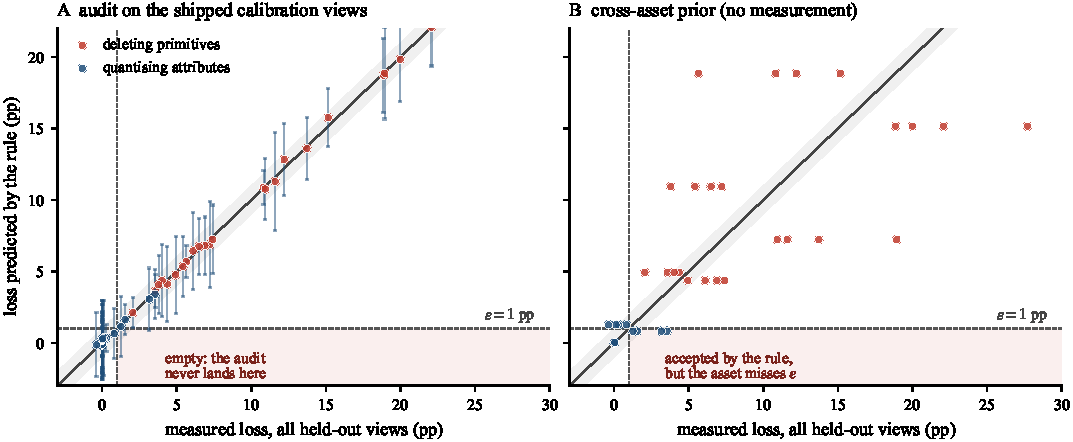
\includegraphics[width=\linewidth]{fig3_audit.pdf}
  \caption{The two decision rules of Table~\ref{tab:decision} on one pair of axes: loss predicted by the rule against
  the loss measured on all held-out views, for the $56$ (asset, edit) cells. Bars in panel A are the audit's per-cell
  error over the $400$ calibration/deployment splits; panel B has none, because a prior is not a measurement. The
  shaded corner is where a rule accepts (predicted loss $\le \varepsilon$) while the asset misses the tolerance at
  $\varepsilon = 1$~pp: the audit never lands there, the prior lands there four times. Both rules are accurate above
  the tolerance; they differ exactly where the guarantee is at stake.}
  \label{fig:audit}
\end{figure}

\subsection{Ablations}
\label{sec:ablation}

Table~\ref{tab:bits} prices bit width one field at a time on a single finetuned model, so that nothing but the field
changes. At the mid-rate point, the most expensive field per byte saved is the quaternion ($-0.29$~dB for
$-6.5\%$ bytes) and the cheapest is opacity ($+0.01$~dB for $-2.4\%$); coarsening three fields together costs
$1.22$~dB for $-16.4\%$. Panel B shows the colour block saturating as in \S\ref{sec:res-container}: from $96$ to $48$
bits costs $0.17$~dB and saves $10.2$~MB, while from $40$ to $32$ bits costs $0.69$~dB and saves only $1.1$~MB.

\subsection{A decibel budget is not a coverage budget}
\label{sec:decibel}

\S\ref{sec:collision} left one question open: if fidelity is an unreliable proxy, how unreliable? Over the
quantisation family, one decibel is worth $0.91$ to $3.86$ coverage points depending on the asset --- a $4.2\times$
spread (\texttt{stump}, $3.77$; \texttt{stump\_i7k}, $3.50$; \texttt{bicycle}, $3.86$; \texttt{flowers\_i7k},
$0.91$). A pipeline that enforces a fidelity budget therefore enforces a coverage budget it does not know, and the
error is not a constant that could be absorbed by a margin: it is a factor of four between assets of the same
kind. This is why the planner of \S\ref{sec:planner} optimises the certified quantity directly rather than proxying
it with decibels.

\begin{figure}[t]
  \centering
  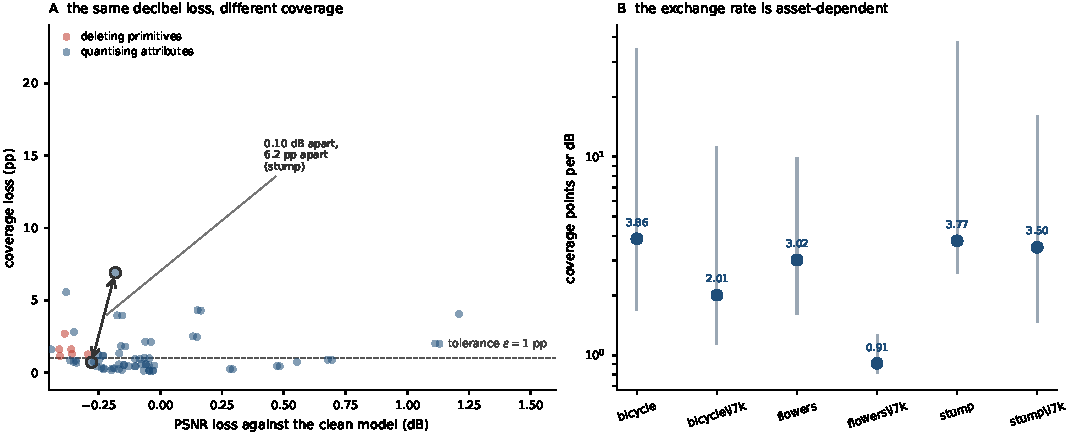
\includegraphics[width=\linewidth]{fig4_decibel.pdf}
  \caption{A decibel budget is not a coverage budget. (A) every configuration of the six usable assets, placed by its
  PSNR loss and by its coverage loss; the circled pair is the widest gap at a matched decibel loss, found from the data
  ($0.10$~dB apart, $6.2$~points apart, \texttt{stump}). (B) the exchange rate per asset, median with the observed
  range: coverage points bought or lost per decibel, $0.91$--$3.86$ in the median and up to two orders of magnitude
  within one asset. A tolerance stated in decibels is therefore a tolerance the sender cannot compute.}
  \label{fig:decibel}
\end{figure}

\subsection{What the bit budget can and cannot buy}
\label{sec:midrate-bound}

The planner's grid in \S\ref{sec:planner} moves three things: the keep fraction, the colour budget and the geometry
budget. It is worth stating why those three and not, say, ``more primitives'', because the answer is a measured
exchange rate that closes the alternative.

Geometry is $9.16$~B of the $13.60$~B per primitive and colour $4.34$~B; the colour block is therefore no longer the
lever it was before \S\ref{sec:res-container}. What does one byte buy? Buying primitives is worth $0.075$~dB per byte:
a $40\%$ increase in primitive count ($1.53$ to $2.15$~M at a fixed keep fraction) buys $+0.57$~dB. Selling geometry
bytes is worth far more, in the wrong direction: the step from \texttt{gp6-6-6\_c8} to \texttt{gp4-4-4\_c6} saves
$2.03$~B per primitive and costs $1.51$~dB, i.e. $0.30$--$0.90$~dB per byte depending on the field
(Table~\ref{tab:bits}). The two rates differ by $4$--$12\times$.

So a byte moved from geometry precision to primitive count always loses, and no reallocation inside this
representation can buy the missing decibels. That is the arithmetic behind \S\ref{sec:published}: the gap to
anchor-based coders is a representation gap, and the planner is not allowed to paper over it by trading precision for
quantity. It spends the budget where the measured exchange rate says the guarantee survives, and refuses when no
configuration in the grid does (Algorithm~\ref{alg:carp}, the refusal branch).

\subsection{What the shipped quantile delivers, per pixel and per view}
\label{sec:viewlevel}

Every number so far scores a compressed asset against a quantile calibrated on the \emph{clean} model, which is what
a recipient actually holds. Table~\ref{tab:viewlevel} and Figure~\ref{fig:viewlevel} ask the next question: at that
fixed $q$, how much of the promise survives, and to whom.

Three answers, and the third is the uncomfortable one.

\emph{Pixel coverage is nearly free to keep, up to a point.} On \texttt{bicycle} the colour ladder holds coverage
between $0.910$ and $0.874$ from $1\times$ out to $10.5\times$; on \texttt{stump} it holds $0.911$ down to $0.906$ at
$8.3\times$ and then collapses to $0.788$ at $10.5\times$. The cliff is real and it moves between assets, which is
the rate--coverage frontier of \S\ref{sec:frontier} seen from the certificate's side.

\emph{The view-level statement is much weaker, before any compression at all.} Even the clean model, at a nominal
$90\%$ pixel guarantee, has only $72\%$ of its held-out views with $90\%$ of their pixels covered. That is the
pixel-versus-view gap VSCP reports, now measured on our own assets rather than cited; we give it as a measured fact
about the quantity we ship, not as a defect of the container.

\emph{The two criteria we set in advance did not both survive.} We expected geometry coarsening to cost at least
$2\times$ the coverage of a colour reduction at a matched rate, on at least three of the four fields. It holds on two
fields for \texttt{bicycle} ($2.7\times$ for 4-bit quaternions, $6.9\times$ for 4-bit scales) and on one for
\texttt{stump} ($5.9\times$ for scales), and the other fields sit at $1.4$--$1.8\times$. The coarse claim of
\S\ref{sec:collision} --- pruning is dominated --- is untouched, because it compares deletion against quantisation at
a matched rate over $12.7$--$23.2$ points; the fine claim, that \emph{every} geometry field is worse per byte than
colour, is not supported at this resolution and is withdrawn here. We also expected the two-view audit to stay within
$3$~pp; it stays within $3.9$--$4.6$~pp on \texttt{bicycle} and $2.9$--$3.2$~pp on \texttt{stump}, i.e. it degrades
from the $2.0$~pp measured on the edit grid (\S\ref{sec:decision}) when the perturbation is a quantisation ladder
rather than a deletion family. Both failures are reported in the deposit with the script that produced them.

\begin{table}[t]
\centering
\small
\footnotesize
\setlength{\tabcolsep}{3.2pt}
\caption{What the shipped quantile actually delivers. The quantile $q$ is calibrated once on the \emph{clean} model's calibration views and then held fixed; every compressed row is scored against that unchanged $q$. \emph{pixel} is the fraction of held-out pixels covered, \emph{view} the fraction of held-out views with at least $90\%$ of their pixels covered, \emph{audit} the error of a two-view audit.}
\label{tab:viewlevel}
\begin{tabular}{llrrrrrr}
\toprule
scene & configuration & MB & rate & PSNR & pixel & view & audit (pp) \\
\midrule
bicycle & \texttt{clean} & 1447.14 & 1.00$\times$ & 24.65 & 0.910 & 0.722 & 3.86 \\
 & \texttt{gp6-6-6\_c8\_sh6} & 285.71 & 5.07$\times$ & 24.58 & 0.908 & 0.722 & 3.90 \\
 & \texttt{gp6-6-6\_c8\_sh4} & 212.13 & 6.82$\times$ & 24.56 & 0.908 & 0.722 & 3.89 \\
 & \texttt{gp6-6-6\_c8\_sh3} & 175.34 & 8.25$\times$ & 24.47 & 0.906 & 0.682 & 3.94 \\
 & \texttt{gp6-6-6\_c8\_sh2} & 138.54 & 10.45$\times$ & 23.54 & 0.874 & 0.521 & 4.55 \\
 & \texttt{gp4-6-6\_c8\_sh3} & 170.74 & 8.48$\times$ & 24.12 & 0.898 & 0.682 & 3.91 \\
 & \texttt{gp6-4-6\_c8\_sh3} & 170.74 & 8.48$\times$ & 23.54 & 0.880 & 0.478 & 4.28 \\
 & \texttt{gp6-6-4\_c8\_sh3} & 173.80 & 8.33$\times$ & 24.36 & 0.902 & 0.682 & 3.89 \\
 & \texttt{gp6-6-6\_c7\_sh3} & 173.04 & 8.36$\times$ & 24.40 & 0.904 & 0.682 & 3.94 \\
\midrule
stump & \texttt{clean} & 1170.98 & 1.00$\times$ & 26.38 & 0.911 & 0.741 & 3.00 \\
 & \texttt{gp6-6-6\_c8\_sh6} & 231.19 & 5.07$\times$ & 26.31 & 0.909 & 0.741 & 2.98 \\
 & \texttt{gp6-6-6\_c8\_sh4} & 171.65 & 6.82$\times$ & 26.29 & 0.909 & 0.741 & 2.97 \\
 & \texttt{gp6-6-6\_c8\_sh3} & 141.88 & 8.25$\times$ & 26.18 & 0.906 & 0.741 & 2.95 \\
 & \texttt{gp6-6-6\_c8\_sh2} & 112.11 & 10.45$\times$ & 23.88 & 0.788 & 0.000 & 2.86 \\
 & \texttt{gp4-6-6\_c8\_sh3} & 138.16 & 8.48$\times$ & 26.11 & 0.904 & 0.741 & 2.96 \\
 & \texttt{gp6-4-6\_c8\_sh3} & 138.16 & 8.48$\times$ & 25.43 & 0.881 & 0.431 & 3.22 \\
 & \texttt{gp6-6-4\_c8\_sh3} & 140.64 & 8.33$\times$ & 26.06 & 0.903 & 0.741 & 2.96 \\
 & \texttt{gp6-6-6\_c7\_sh3} & 140.02 & 8.36$\times$ & 26.08 & 0.903 & 0.741 & 2.96 \\
\bottomrule
\end{tabular}
\end{table}


\begin{figure}[t]
  \centering
  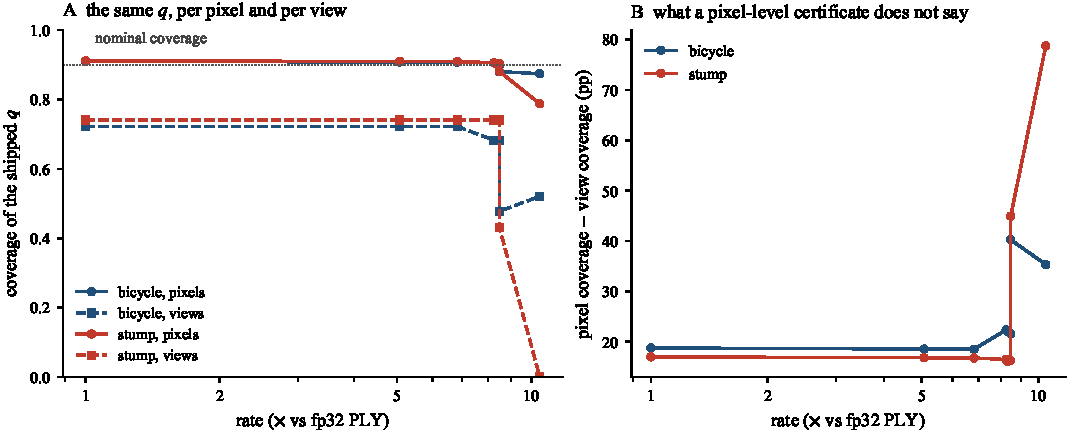
\includegraphics[width=\linewidth]{fig5_viewlevel.pdf}
  \caption{The shipped quantile, held fixed, re-measured as the container spends fewer bytes. (A) solid: fraction of
  held-out pixels covered; dashed: fraction of held-out views with at least $90\%$ of their pixels covered. (B) the
  distance between the two. The pixel statement is robust to about $8\times$; the view statement is already $18$--$19$
  points below it on the clean model, and the gap widens to $35$--$79$ points at $10\times$.}
  \label{fig:viewlevel}
\end{figure}

\subsection{What the compression looks like}
\label{sec:qualitative}

Figure~\ref{fig:qualitative} puts the two families on one held-out view of \texttt{bicycle}, at a magnification chosen
by rule rather than by eye: the view is the one whose clean PSNR is the median over the deployment views, and the
patch is the $200\times200$ ground-truth window with the largest gradient energy --- both fixed before the renders
existed, so the patch that is magnified is not the patch that fails.

Read the top row as a viewer would. At $5.07\times$ ($26.84$~dB) and $8.25\times$ ($26.59$~dB) the container is hard
to separate from the clean render; the Fisher prune at half the primitives ($2.00\times$, a quarter of the saving) is
the only arm whose structure visibly changes in the same window, and it is also the arm with the lowest PSNR
($26.11$ against $26.59$ at $8.25\times$ and $27.03$ for the clean model). The bottom row isolates the \emph{action} by
differencing each render against the clean one, amplified $8\times$: quantisation spreads its error over texture, while
pruning concentrates its error on the slat edges --- which is what deleting primitives means geometrically. The figure
therefore restates the asymmetry of \S\ref{sec:frontier} in a currency a reader can check without trusting our
metrics.

The numbers in that row are one view, not a scene mean, so they are not comparable with the \texttt{bicycle} rows of
Table~\ref{tab:viewlevel}: this view's clean PSNR ($27.03$~dB) sits $2.4$~dB above the scene mean. Only the ordering
within the figure is claimed.

\begin{figure}[t]
  \centering
  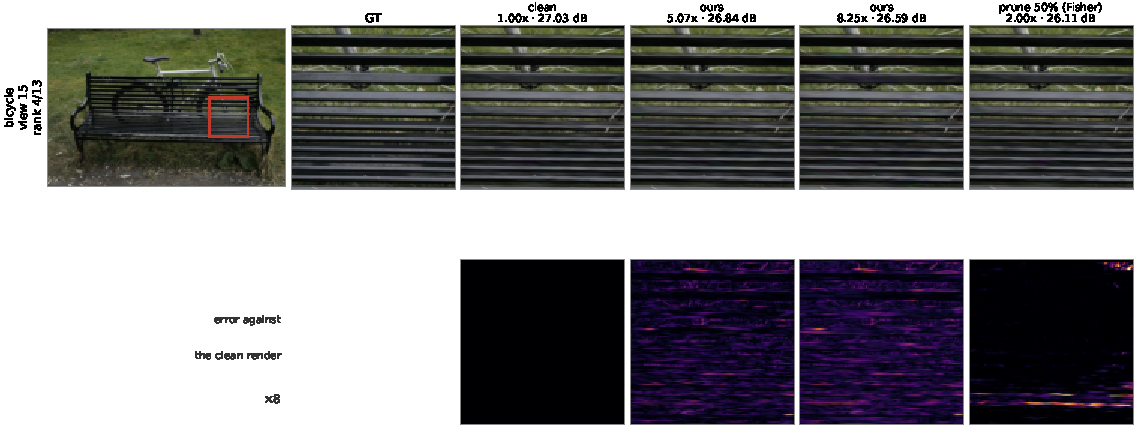
\includegraphics[width=\linewidth]{fig6_qualitative.pdf}
  \caption{The same view, four ways. Top: the held-out view whose clean PSNR is the median of the deployment views
  (rank $4/13$), with the magnified window marked; the window is the ground-truth $200\times200$ patch with the largest
  gradient energy. Bottom: each arm differenced against the \emph{clean} render, amplified $8\times$, so the panel shows
  what the action did rather than how far the model is from the ground truth. At $8.25\times$ the container's error is
  distributed over texture; at $2.00\times$ the prune's error is concentrated on edges.}
  \label{fig:qualitative}
\end{figure}

\begin{table}[t]
\centering
\small
\footnotesize
\setlength{\tabcolsep}{2.8pt}
\caption{Same model, same container, five pruning scores at half the primitives (\texttt{bonsai}, 1{,}244{,}819 primitives). BD-rate is measured on \texttt{bicycle} over four colour budgets without finetuning.}
\label{tab:prune}
\begin{tabular}{lrrrr}
\toprule
arm & primitives & file & PSNR & $\Delta$PSNR \\
\midrule
control (no prune) & 1,244,819 & 15.30 MB & 27.08 & -- \\
fisher & 622,410 & 8.07 MB & 26.58 & -0.50 \\
opacity & 622,410 & 7.95 MB & 26.15 & -0.93 \\
area & 622,410 & 7.84 MB & 24.92 & -2.16 \\
volume & 622,410 & 7.84 MB & 24.55 & -2.53 \\
\midrule
BD-rate, fisher & \multicolumn{3}{r}{-45.06\,\%} (4 points) \\
BD-rate, opacity & \multicolumn{3}{r}{-44.96\,\%} (4 points) \\
\bottomrule
\end{tabular}
\end{table}


\subsection{Pruning, priced}
\label{sec:pruning}

Because \S\ref{sec:frontier} says pruning is not admissible inside a tight tolerance, it is worth saying what pruning
\emph{is} good for, and what the choice of score is worth. Table~\ref{tab:prune} holds the model, the container and the
keep fraction fixed and varies only the score. The Fisher-diagonal score \cite{pup3dgs} is the best of five and costs
$0.50$~dB for half the primitives on \texttt{bonsai} ($0.53$~dB on \texttt{bicycle}); the viewer's opacity score costs
$0.93$ and $1.28$; the volume proxy that this project used for several rounds costs $2.53$ and $4.39$~dB and is simply
a broken arm. Measured as BD-rate over four colour budgets without finetuning, pruning to half the primitives is worth
$-45.06\%$ of the bitrate with the Fisher score and $-44.96\%$ with opacity --- statistically the same rate, with the
Fisher score buying a higher quality ceiling ($+0.8$~dB). The LPIPS ordering agrees with PSNR and SSIM ($+0.010$ for
the Fisher arm against $+0.096$ for the volume arm at half the bytes), so the score comparison is not an artefact of
one metric.

\begin{table}[t]
\centering
\small
\footnotesize
\setlength{\tabcolsep}{2.8pt}
\caption{Perceptual metrics at half the bytes on one model (\texttt{bicycle}, 48-bit colour, LPIPS with a VGG backbone). Every arm keeps the same container; only the pruning score changes.}
\label{tab:perceptual}
\begin{tabular}{lrrrrr}
\toprule
arm & file & PSNR & SSIM & LPIPS & $\Delta$LPIPS \\
\midrule
control (no prune) & 76.60 MB & 24.06 & 0.7393 & 0.2813 & +0.0000 \\
fisher & 40.17 MB & 23.52 & 0.7269 & 0.2916 & +0.0103 \\
opacity & 39.50 MB & 22.78 & 0.7049 & 0.3034 & +0.0221 \\
area & 39.00 MB & 22.14 & 0.6662 & 0.3264 & +0.0451 \\
volume & 38.76 MB & 19.67 & 0.5782 & 0.3777 & +0.0964 \\
\bottomrule
\end{tabular}
\end{table}


Table~\ref{tab:perceptual} closes the loop on the score question with a perceptual metric rather than PSNR. Half the
bytes costs $+0.010$ LPIPS with the Fisher score and $+0.096$ with the volume proxy, and the ordering of the five arms
is identical under PSNR, SSIM and LPIPS --- so \S\ref{sec:pruning}'s conclusion is not an artefact of one metric. It is
also the honest place to say what this table does \emph{not} establish: LPIPS is a proxy, we ran no subjective study,
and the compressed-3DGS perceptual literature has its own datasets and protocols for that question
\cite{gscompqa,gsbench}.

\begin{table}[t]
\centering
\small
\footnotesize
\setlength{\tabcolsep}{2.8pt}
\caption{Decode cost measured end to end (container $\rightarrow$ tensors), Peak is the decoder's peak resident memory. The last four rows are the encoder side on \texttt{bicycle}.}
\label{tab:cost}
\begin{tabular}{llrrrr}
\toprule
scene & spec & file & decode (s) & peak (GB) & PSNR \\
\midrule
bicycle & \texttt{gp6-6-6\_c8} & 76,598,203 B & 15.95 & 4.27 & 24.06 \\
bicycle & \texttt{gp6-6-4\_c8} & 74,802,867 B & 15.76 & 4.27 & 23.95 \\
stump & \texttt{gp6-6-6\_c8} & 62,649,653 B & 12.85 & 3.49 & 25.52 \\
stump & \texttt{gp6-6-4\_c8} & 61,191,922 B & 12.72 & 3.49 & 25.41 \\
bonsai & \texttt{gp6-6-6\_c8} & 15,297,685 B & 3.25 & 0.95 & 27.08 \\
bonsai & \texttt{gp6-6-4\_c8} & 14,927,795 B & 3.22 & 0.95 & 26.97 \\
\midrule
\multicolumn{2}{l}{encode r=16 / 48 bit (one SVD + allocation + container)} & -- & 51.50 & -- & -- \\
\multicolumn{2}{l}{decode r=16 / 48 bit} & -- & 9.16 & -- & -- \\
\multicolumn{2}{l}{decode + PLY write} & -- & 15.90 & -- & -- \\
\multicolumn{2}{l}{render, 25 held-out views} & -- & 10.60 & -- & -- \\
\bottomrule
\end{tabular}
\end{table}


\subsection{Cost}
\label{sec:cost}

Table~\ref{tab:cost} is the accounting a deployment needs. Decoding \texttt{bicycle} at $76.60$~MB takes $15.95$~s
and $4.27$~GB of resident memory; the smaller scenes scale down (\texttt{bonsai}: $3.25$~s, $0.95$~GB). Encoding the
near-lossless point costs $51.5$~s of one-time work (one SVD, one allocation pass, one container write) and decoding
it $9.16$~s, both dominated by I/O rather than arithmetic. Rendering $25$ held-out views at $1236 \times 822$ takes
$10.6$~s, which is the number that matters for the audit: one pass is cheap enough to be a deployment step rather
than an evaluation ritual.

\begin{table}[t]
\centering
\small
\footnotesize
\setlength{\tabcolsep}{2.8pt}
\caption{Our best row at or below each published file size. Positive gap = we are behind. The published numbers are transcribed in \texttt{experiments/published\_3dgs.json}; the 0.55 dB protocol bias measured in M16 is stated, not folded in.}
\label{tab:gap}
\begin{tabular}{llrrrrr}
\toprule
scene & method & their file & their PSNR & our file & our PSNR & gap (dB) \\
\midrule
bicycle & 3DGS & 1336.45 MB & 25.11 & 278.50 MB & 24.49 & +0.62 \\
bicycle & HAC & 27.54 MB & 25.05 & 25.67 MB & 22.08 & +2.97 \\
bicycle & PCGS & 19.09 MB & 25.12 & 18.40 MB & 21.50 & +3.62 \\
stump & HAC & 18.11 MB & 26.58 & 17.61 MB & 20.33 & +6.25 \\
bicycle & CompGS & 47.15 MB & 24.97 & 25.67 MB & 22.08 & +2.89 \\
bicycle & EAGLES & 104.00 MB & 25.04 & 83.41 MB & 24.08 & +0.96 \\
\bottomrule
\end{tabular}
\end{table}


\subsection{Where we lose}
\label{sec:published}

Table~\ref{tab:gap} is computed, not narrated: our best row at or below each published file size, against the
published PSNR. On \texttt{bicycle} we are $0.62$~dB behind the uncompressed 3DGS point at $278.50$~MB, $2.97$~dB
behind HAC at $25.67$~MB, $3.62$~dB behind PCGS at $18.40$~MB, $2.89$~dB behind CompGS at $25.67$~MB, and $0.96$~dB
behind EAGLES \cite{eagles} at $83.41$~MB; on \texttt{stump} the HAC gap is $6.25$~dB. Two rules make the table
reproducible: each
published method enters at the operating point its authors report for that scene (HAC's lower-rate setting,
$27.54$~MB, rather than its $39.15$~MB one; PCGS at $\lambda_s = 4\times10^{-4}$; CompGS and EAGLES as published), and
a method is excluded only when it reports no per-scene file size, which is the case for LightGaussian
\cite{lightgaussian}. The $0.55$~dB
protocol bias measured in \S\ref{sec:assets} does not close any of these gaps.

The cause is representational and we state it in the same terms the numbers do: an anchor-based coder spends $3$--$6$~B
per primitive on a residual against a learned anchor while we spend $9.16$~B on geometry plus $4.34$~B on colour,
because every primitive pays for its own SH coefficients. A rebuild along those lines was attempted inside this
project and stopped at a pre-registered gate when the prototype's anchor-conditioned prediction could not pay for the
anchor it needed; we report the gate rather than the aspiration.

%% =====================================================================
\section{Limitations and future work}
\label{sec:limits}

\paragraph{The fidelity gap is real.} \S\ref{sec:published} quantifies it and this paper does not close it.
Reconstruction-aware coding --- anchors plus an in-loop quantiser, which is what HAC and PCGS do --- is the route, and
it is a different paper's worth of training infrastructure. Until then our claims are about guarantee-preserving rate
reduction at the near-lossless and mid-rate operating points we measure, not about the fidelity frontier.

\paragraph{Two scenes carry the cross-paper rows.} Only \texttt{bicycle} and \texttt{stump} reproduce the published
3DGS number closely enough to compare against HAC and PCGS; the other six scene-checkpoints are internal. The
exclusion rule is mechanical (\S\ref{sec:assets}) and the reason is a protocol difference, but a reader should treat
the published-format collision in \S\ref{sec:frontier} as the generalisable evidence and the HAC/PCGS rows as
indicative.

\paragraph{The envelope is empirical.} Equation~\eqref{eq:envelope} is a supremum over a finite sample; a DKW band at
our sample sizes is of the same order as the statistic. We therefore report the envelope's measured tightness
($0.64$ median) and its $56/56$ validity rather than a finite-sample level, and the audit --- not the envelope --- is
the operative check.

\paragraph{Per-pixel coverage is not a view-level guarantee, and we now measure the gap.} VSCP \cite{vscp} shows
that pixel-pooled calibration can hit its nominal level while the view-level event is far below it. Our own assets
agree, and worse: the clean model's nominal $90\%$ pixel statement holds for $72\%$ of views, and at $10\times$
(Table~\ref{tab:viewlevel}) the view-level fraction falls to $0.00$ on \texttt{stump} while pixel coverage is still
$0.79$. We nonetheless plan against the per-pixel quantity, because it is what a shipped certificate names and what
the tolerance is defined on; a view-level certificate would need its own audit and would move every number in
\S\ref{sec:frontier}. What changes with this measurement is that the cost of that choice is now stated in points, not
in a citation.

\paragraph{The audit has a resolution, and we now state it.} Its single-pass error is $2.0$ points against a tolerance we usually set at $1$~pp (\S\ref{sec:decision}). The $56/56$ of Table~\ref{tab:decision} is the split-averaged decision; a single pass would mis-decide the cells that sit inside that error, and Table~\ref{tab:abstain} prices the abstention band that removes them. A recipient who needs a verdict at $\pm1$~pp must ship more calibration views, not a better estimator.

\paragraph{No subjective study.} LPIPS and SSIM are proxies; the perceptual literature for compressed 3DGS now has
its own datasets and subjective protocols \cite{gscompqa,gsbench}. A subjective check of the frontier points is the
natural next experiment, and we would expect the tolerance to move rather than the ranking to change.

%% =====================================================================
\section{Conclusion}
\label{sec:conclusion}

A 3DGS asset now changes hands, and the guarantee that travels with it is only as good as what the next owner does to
the file. This paper makes that statement quantitative and then makes it actionable. Quantitatively, the damage an
edit does to a shipped coverage certificate is decided by the edit family: geometric edits cost $12.7$--$23.2$ points
at a matched rate, attribute edits cost $0.7$--$0.95$, and inside a one-point tolerance the pruning family has no
admissible operating point at all. Actionably, the three pieces a sender needs are cheap: a container that makes
attribute quantisation worth spending ($17.35\times$ at $-0.04$~dB), an audit that turns the certificate into
something a recipient can check with one render pass ($2.0$ points of error, no new labels), and a planner whose
acceptance test is that audit --- because the prior alone ships a broken guarantee on two to three assets out of six.

\section*{CRediT authorship contribution statement}

\textbf{Tianji Su}: Conceptualization, Methodology, Software, Validation, Formal analysis, Investigation, Data
curation, Writing -- original draft, Writing -- review \& editing, Visualization.

\section*{Declaration of competing interest}

The author declares that he has no known competing financial interests or personal relationships that could have
appeared to influence the work reported in this paper.

\section*{Data availability}

The code, the per-view residual dumps, the derived tables and the reproduction scripts that support this study are
archived at Zenodo under DOI \TBD{Zenodo DOI}, maintained at
\url{https://github.com/11qishiyi/care-gs} (release \texttt{v1.0.0}), and permanently snapshotted at
Software Heritage (\texttt{swh:1:snp:dc2330759abf7709dba3573f8a3a87fb74361575}). Every number in
Tables~\ref{tab:container}--\ref{tab:gap} is regenerated from those artefacts by the scripts in the archive.

\section*{Declaration of generative AI and AI-assisted technologies}

During the preparation of this work the author used an AI assistant for language editing and for drafting
code-review notes. The author reviewed and edited the content and takes full responsibility for the content of the
published article. No experimental image or table value was generated by an AI tool.

\bibliographystyle{elsarticle-num}
\bibliography{refs}

\end{document}
